% !Mode:: "TeX:UTF-8"
% VL 7, gebaut aus part-lernen/11-aktivierungsfunktionen.md, 12-netze-von-hand.md
% und 13-universelle-approximation.md
% (Dialogmuster: transcripts/vl06-backprop-2025 (Aktivierungen) und
%  transcripts/vl07-netze-von-hand-autoencoder-2025/notiz.md).
% !Mode:: "TeX:UTF-8"
\newcommand{\thepage}{} % to silence a hyperref warning about pdfpagelabels
\RequirePackage[]{silence}
\WarningsOff[hyperref]
\PassOptionsToPackage{log-declarations=false}{xparse}
%\RequirePackage[l2tabu, orthodox]{nag}
\RequirePackage{luatex85} % to make \pdf...= commands work with LuaTeX
\documentclass[aspectratio=169,t]{beamer}
\usepackage{ifthen}
\usepackage[T1]{fontenc}
\usepackage{iftex}
\ifLuaTeX
 \usepackage{fontspec}
 \setmainfont[Ligatures=TeX]{Source Sans Pro}
\else
 \usepackage[utf8]{inputenc}
\fi
\usepackage{german}
\usepackage{newunicodechar}
\newunicodechar{€}{\texteuro}
\newunicodechar{ß}{\ss}
\renewcommand{\SS}{\iffontchar\font"1E9E \symbol{"1E9E}\else SS\fi}
\usepackage{ellipsis}
\usepackage{microtype}
\usepackage{listings}
\usepackage{sourcecodepro}
\lstset{language=Python, basicstyle=\ttfamily}
\usepackage{amsfonts}
\usepackage{amssymb}
\usepackage{amsthm}
\usepackage{fancyhdr}
\usepackage{graphicx}

\newtheorem{proposition}[theorem]{Proposition}

\DeclareMathOperator*{\argmax}{argmax}
\DeclareMathOperator{\supp}{supp}
\newcommand{\E}{\ensuremath{\mathbb{E}}}
\newcommand{\V}{\ensuremath{\mathbb{V}}}

\setbeamercolor{emph}{fg=purple}
\renewcommand<>{\emph}[1]{%
  {\usebeamercolor[fg]{emph}\only#2{\itshape}#1}%
}



\hypersetup{draft=false,colorlinks=false,pdfpagemode=UseOutlines,plainpages=false,
            breaklinks=true,bookmarksnumbered=true,pdfborder=0 0 0,
            pdftitle={Einführung in Deep Learning WiSe 2026/27 HHU},
            pdfauthor={Konrad Voelkel},
            pdfsubject={data science}}

%\documentclass[aspectratio=169,t]{beamer}
\usetheme{hhubeamer} % put the hhu-beamer-theme in /usr/share/texmf/tex/latex/beamer/themes/

% -------------------- Code listings config --------------------
% Define custom colors for syntax highlighting
\definecolor{codegreen}{rgb}{0,0.6,0}
\definecolor{codegray}{rgb}{0.5,0.5,0.5}
\definecolor{codepurple}{rgb}{0.58,0,0.82}
\definecolor{backcolour}{rgb}{0.96,0.96,0.94} % Very light gray/beige
% Configure the listings package
\lstset{
    language=Python,
    backgroundcolor=\color{backcolour},   
    commentstyle=\color{codegreen}\itshape,
    keywordstyle=\color{blue}\bfseries,
    numberstyle=\tiny\color{codegray},
    stringstyle=\color{codepurple},
    basicstyle=\ttfamily\footnotesize, % Use a monospaced font
    breakatwhitespace=false,         
    breaklines=true,      
             % Enable automatic line breaking
    captionpos=b,                      % Caption at the bottom
    keepspaces=true,                 
    numbers=left,                      % Line numbers on the left
    numbersep=10pt,                    % Distance of line numbers from the code
    showspaces=false,                
    showstringspaces=false,            % Don't show weird underscores in strings
    showtabs=false,                  
    tabsize=4,
    frame=single,                      % Add a subtle border around the code
    rulecolor=\color{black!20},        % Border color
  }

\event[]{}
\author[Wintersemester 2026/27]{Dr. Konrad Völkel, Wintersemester 2026/27}

%\title{Data Science, VL 1}
%\date{16.04.2026}


%%% Local Variables:
%%% mode: latex
%%% TeX-master: t
%%% End:


% Fassung mit Dozentennotizen (zweiter Schirm): die nächste Zeile einkommentieren.
% \setbeameroption{show notes on second screen=right}

\graphicspath{{../images/}}

\title[Netze von Hand (VL 7)]{Aktivierungsfunktionen und Netze von Hand\\\large Einführung in Deep Learning, VL 7}
\date{25.11.2026}

\begin{document}

\begin{frame}
  \titlepage

  \note{\textbf{Ablauf, 90 Minuten.} Drei Kapitel, die 2025 auf zwei Sitzungen verteilt
    waren (Aktivierungen im Backprop-Termin, Netze von Hand danach):\\[2pt]
    \begin{tabular}{@{}rll@{}}
      0--4   & Folie 2       & Rückblick: was noch fehlt\\
      4--16  & Folien 3--5   & ReLU, warum sie passt\\
      16--26 & Folien 6--7   & Sterbende Neuronen, ELU/Swish/GELU\\
      26--40 & Folien 8--10  & Boolesche Netze: NOT, OR, NOR\\
      40--52 & Folien 11--12 & XOR als Schnitt, Playground-Lösungen\\
      52--68 & Folien 13--15 & \textbf{$x^2$ aus ReLUs bauen}, dann $xy$\\
      68--82 & Folien 16--18 & Universelle Approximation\\
      82--90 & Folien 19--20 & Take-Home, Blatt 7\\
    \end{tabular}\\[4pt]
    \textbf{Diese Sitzung lebt vom Hörsaaldialog} --- die Booleschen Netze und $x^2$
    gemeinsam bauen, nicht vortragen. 2025 war „geometrisch programmieren“ die Formel,
    die gezündet hat. Drei Viertelstunden dafür einplanen.}
\end{frame}

\begin{frame}
  \frametitle{Was wir haben --- und was fehlt}

  \begin{columns}[t]
    \begin{column}{0.48\textwidth}
      \textbf{Haben:}
      \begin{itemize}
      \item Neuron = Skalarprodukt + $\tau$
      \item Gradientenabstieg
      \item Backpropagation
      \end{itemize}
    \end{column}
    \begin{column}{0.48\textwidth}
      \textbf{Fehlt:}
      \begin{itemize}
      \item Welches $\tau$?
      \item Gibt es die Gewichte überhaupt?
      \end{itemize}
    \end{column}
  \end{columns}

  \note{Die zweite Frage ist die interessantere und der rote Faden heute: Bevor wir einem
    Optimierer zutrauen, Gewichte zu \emph{finden}, überzeugen wir uns, dass es sie
    \emph{gibt} --- indem wir sie von Hand hinschreiben.}
\end{frame}

% ------------------------------------------------------------------ ReLU
\begin{frame}
  \frametitle{Neues Ziel: Funktionen lernen}

  \begin{center}
    \Large
    Bisher: Klassifikation.\\[12pt]
    Jetzt: eine Funktion lernen --- stückweise linear.
  \end{center}

  \bigskip
  \begin{center}
    Welches $\tau$ ist dafür geeignet?
  \end{center}

  \note{Frage in den Raum stellen und Vorschläge sammeln, bevor die nächste Folie kommt.
    Sigmoid ist die naheliegende Antwort und die falsche für diesen Zweck.}
\end{frame}

\begin{frame}
  \frametitle{ReLU}

  \begin{center}
    \Huge $\operatorname{ReLU}(y) = \max(0, y)$
  \end{center}

  \bigskip
  \begin{center}
    \normalsize Ableitung: 1 für $y > 0$, 0 für $y < 0$, \emph{definiert} als 0 bei $y = 0$.
  \end{center}

  \note{Dass man die Ableitung an einer Stelle einfach festlegen darf, ist genau der
    Inhalt von Blatt 3: schwache Ableitungen dürfen an einzelnen Punkten beliebig sein.
    Die Wahl 0 statt 1 spart Rechnungen.
    Name: \emph{Rectified} Linear Unit --- Gleichrichter, wie in der Elektrotechnik.}
\end{frame}

\begin{frame}
  \frametitle{Warum ReLU passt}

  \begin{columns}[c]
    \begin{column}{0.46\textwidth}
      \Large
      Linear + ReLU\\[8pt]
      $=$ Projektion auf einen Halbraum\\[14pt]
      \normalsize Summe von Knicken\\ $=$ stückweise linear
    \end{column}
    \begin{column}{0.5\textwidth}
      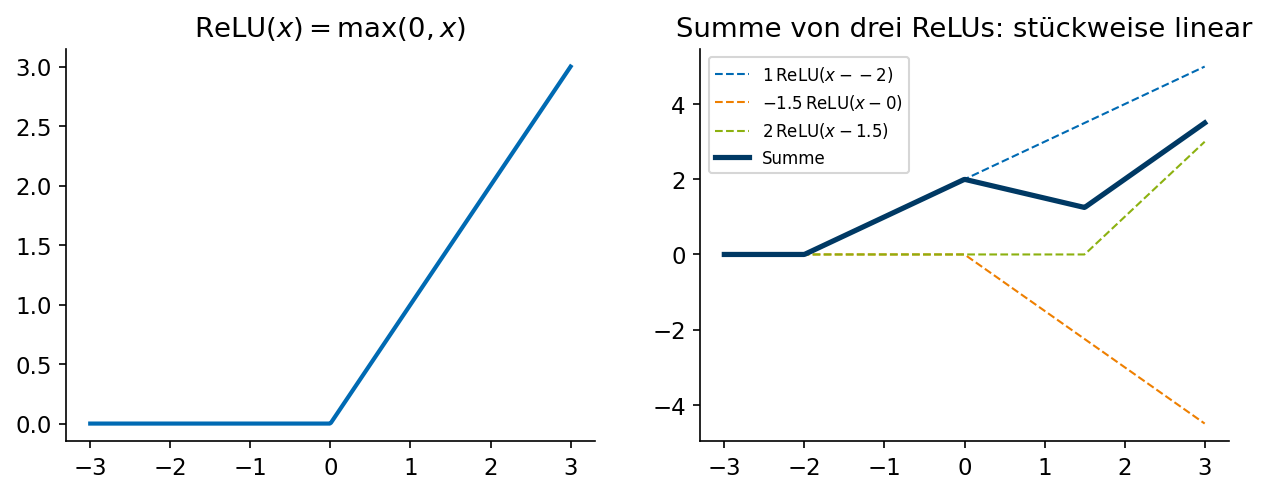
\includegraphics[width=\textwidth]{vl06-relu-sum.png}
    \end{column}
  \end{columns}

  \note{Ein ReLU-Neuron $\max(0, \langle w,x\rangle + b)$ ist null auf der einen Seite der
    Hyperebene und steigt linear auf der anderen. Die Knickstelle \emph{ist} die
    Hyperebene.
    Summiert man solche Knickfunktionen mit Gewichten, bekommt man stückweise lineare
    Funktionen --- und damit lässt sich jede stetige Funktion approximieren. Das bauen
    wir gleich.}
\end{frame}

\begin{frame}
  \frametitle{Problem: sterbende Neuronen}

  \begin{center}
    \Large
    Eingabe immer negativ $\;\Rightarrow\;$ Ausgabe immer 0\\[10pt]
    $\Rightarrow$ Ableitung 0 $\;\Rightarrow\;$ $\delta = 0$\\[10pt]
    $\Rightarrow$ die Gewichte ändern sich nie wieder.
  \end{center}

  \note{Das Neuron ist tot. Mit dem Bild aus VL 6: Das Fehlersignal kommt dort nicht mehr
    an, weil es mit null multipliziert wird.
    Bild vom flachen Land: Wer im flachen Gelände steht, bekommt vom Gradienten keine
    Richtung mehr.}
\end{frame}

\begin{frame}
  \frametitle{Zwei Auswege}

  \begin{columns}[c]
    \begin{column}{0.46\textwidth}
      \Large
      Leaky ReLU, ELU\\[8pt]
      \normalsize im Negativen nicht ganz flach\\[16pt]
      \Large Swish, GELU\\[8pt]
      \normalsize glatt: $y\,\sigma(y)$, \; $y\,\Phi(y)$
    \end{column}
    \begin{column}{0.5\textwidth}
      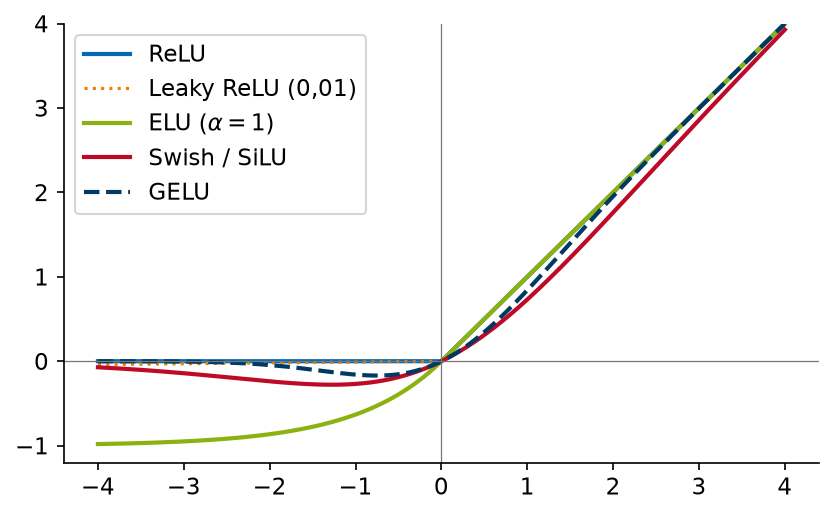
\includegraphics[width=\textwidth]{vl06-activations.png}
    \end{column}
  \end{columns}

  \note{GELU ist heute die Standardwahl in Transformern.
    Am Plot diskutieren, was man eigentlich will: das Signal im Negativen \emph{behalten},
    ohne die Nichtlinearität zu verlieren. Die kleine Delle unter der Achse ist gewollt.
    Swish sieht aus wie das Nike-Logo --- das merkt sich der Hörsaal.}
\end{frame}

% ------------------------------------------------------------------ Boolesche Netze
\begin{frame}
  \frametitle{Von Hand bauen: NOT}

  \begin{center}
    \Huge $n(x) = 1 - x$
  \end{center}

  \bigskip
  \begin{center}
    \normalsize Ein Neuron: Gewicht $-1$, Bias $+1$, Aktivierung $\operatorname{id}$.
  \end{center}

  \note{Interpretation festlegen: $x \le 0$ heißt FALSE, $x \ge 1$ heißt TRUE.
    Wichtig und oft übersehen: Ein Netz ist auf \emph{ganz} $\mathbb{R}$ definiert, nicht
    nur auf den Booleschen Werten. Wir müssen also interpolieren (was ist $n(0{,}5)$?)
    \emph{und} extrapolieren (was ist $n(-1)$?).}
\end{frame}

\begin{frame}
  \frametitle{OR}

  \begin{center}
    \Large
    Ansatz $x + y$? \quad Nein: $f(1,1) = 2$.\\[14pt]
    $[x + y > 0]$ \quad oder besser\\[10pt]
    \Huge $\operatorname{ReLU}(x) + \operatorname{ReLU}(y)$
  \end{center}

  \note{Den ersten Ansatz bewusst scheitern lassen --- der Hörsaal findet den Fehler
    sofort, und das ist der beste Einstieg.
    ReLU schneidet Negatives sauber ab, deshalb die letzte Variante.
    Frage: Was macht diese Funktion bei $(-1, 2)$? Das ist Extrapolation, und wir
    entscheiden sie mit der Wahl der Bausteine.}
\end{frame}

\begin{frame}
  \frametitle{OR und NOR auf ganz $\mathbb{R}^2$}

  \begin{center}
    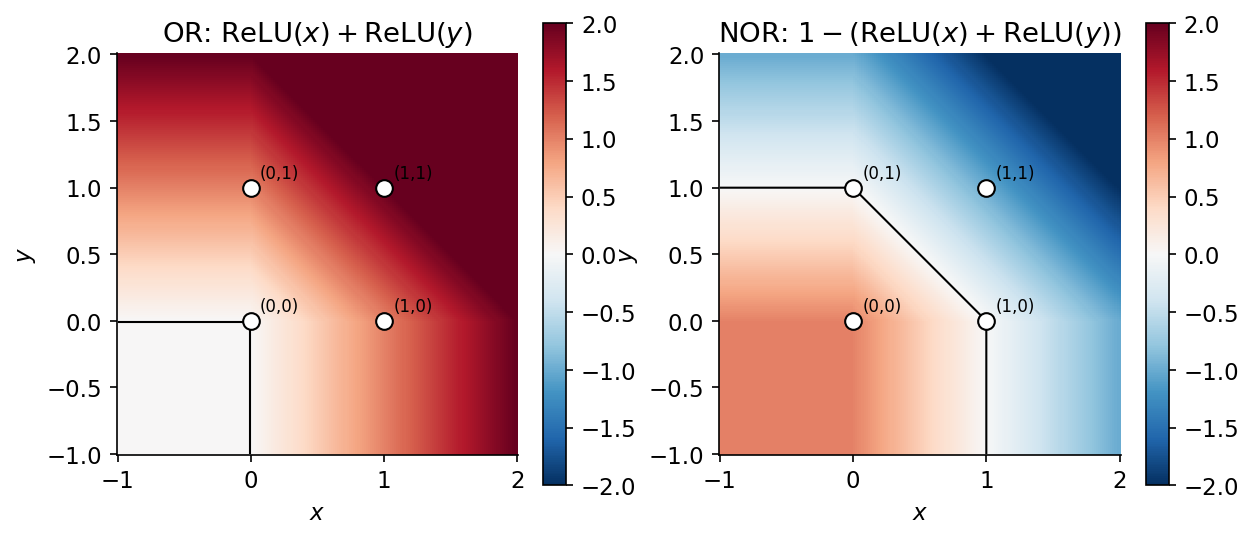
\includegraphics[width=0.66\textwidth]{vl07-or-nor-heatmap.png}
  \end{center}

  \note{Die vier Booleschen Ecken sind markiert, die schwarze Linie ist die
    Nullstellenmenge.
    NOR ist NOT OR, also einfach hintereinandergesetzt:
    $g(x,y) = 1 - (\operatorname{ReLU}(x) + \operatorname{ReLU}(y))$ --- erste Schicht
    ReLU, zweite Schicht Gewicht $-1$, Bias 1.
    \emph{Geometrisch programmieren}: Man legt Hyperebenen in die Ebene und kombiniert
    die Seiten. Das ist die Formel, die 2025 gezündet hat.}
\end{frame}

\begin{frame}
  \frametitle{XOR}

  \begin{columns}[c]
    \begin{column}{0.46\textwidth}
      \Large
      XOR $=$ AND(NAND, OR)
    \end{column}
    \begin{column}{0.5\textwidth}
      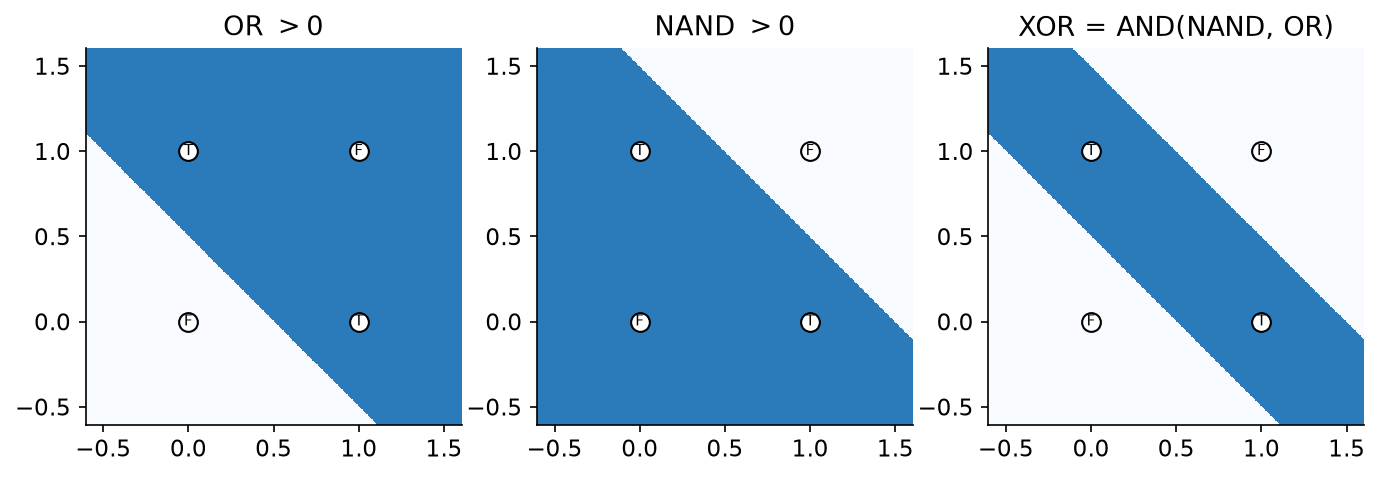
\includegraphics[width=\textwidth]{vl07-xor-region.png}
    \end{column}
  \end{columns}

  \note{Die XOR-Region ist der Schnitt der NAND-Region mit der OR-Region --- zwei
    Halbebenen schneiden.
    Setzt man das mit unseren Bausteinen zusammen, käme man auf 4 versteckte Schichten zu
    je 4 Neuronen. Der Gradientenabstieg findet es mit weniger.}
\end{frame}

\begin{frame}
  \frametitle{Was der Optimierer daraus macht}

  \begin{columns}[c]
    \begin{column}{0.48\textwidth}
      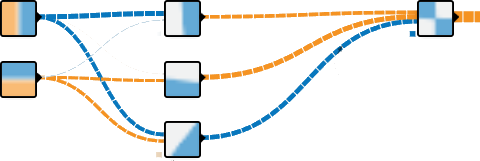
\includegraphics[width=\textwidth]{vl07-xor-playground-3hidden.png}
    \end{column}
    \begin{column}{0.48\textwidth}
      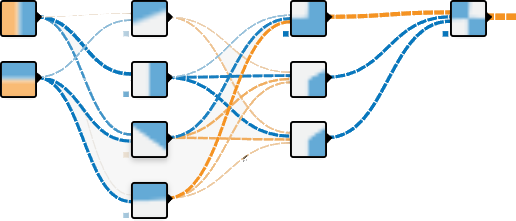
\includegraphics[width=\textwidth]{vl07-xor-playground-2hidden.png}
    \end{column}
  \end{columns}

  \note{Links drei versteckte Schichten, rechts zwei --- beides Approximationen, die der
    Gradientenabstieg im Playground gefunden hat.
    Take-Home: Der Optimierer findet meist \emph{krumme} Gewichte, die trotzdem
    funktionieren, nimmt Abkürzungen und verschwendet Platz (überflüssige Neuronen).
    Wer die Spielaufgabe gemacht hat, kann berichten.}
\end{frame}

% ------------------------------------------------------------------ Arithmetik
\begin{frame}
  \frametitle{Und jetzt Arithmetik}

  \begin{center}
    \Large
    Wie berechnet ein Netz $x^3 + xy^2 - 3y$?\\[16pt]
    \normalsize Zuerst das einfachere Problem: $x^2$.
  \end{center}

  \note{Der Hörsaal soll die Zerlegung vorschlagen: Wenn ich $x^2$ und $xy$ kann und
    addieren kann, habe ich alle Polynome.}
\end{frame}

\begin{frame}
  \frametitle{$x^2$ aus ReLUs}

  \begin{center}
    \Large
    $Q(x) = 9 - 5\operatorname{ReLU}(x+3) + \sum_{k=-2}^{2} 2\operatorname{ReLU}(x-k)$
  \end{center}

  \bigskip
  \begin{center}
    \normalsize Probe: $Q(0) = 9 - 15 + 2\cdot 3 = 0$, \quad $Q(3) = 9 - 30 + 2 \cdot 15 = 9$.
  \end{center}

  \note{\textbf{Gemeinsam entwickeln, nicht vorlesen.} Die Interpolation durch $(k, k^2)$
    hat auf $[k, k+1]$ die Steigung $2k+1$ --- an jeder Stützstelle wächst die Steigung
    um 2, und jeder Knick ist eine ReLU.
    Das ist ein Netz mit einer versteckten Schicht aus 6 ReLU-Neuronen und einer linearen
    Ausgabeschicht.}
\end{frame}

\begin{frame}
  \frametitle{Die Interpolation}

  \begin{center}
    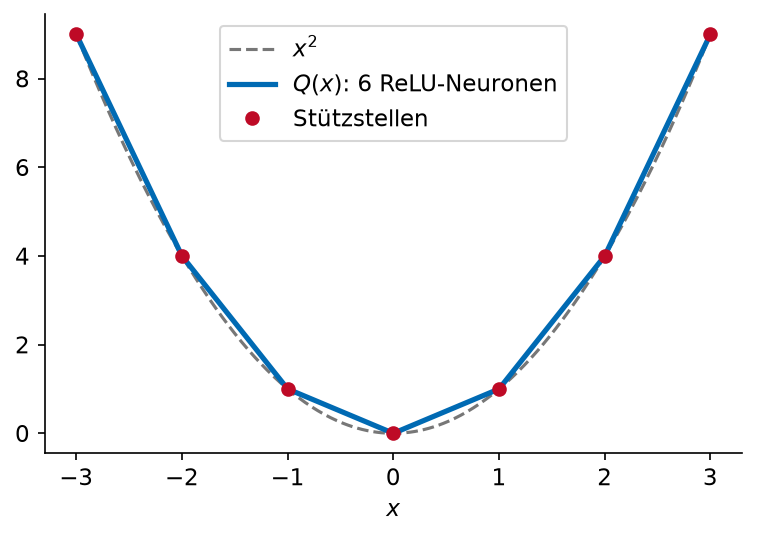
\includegraphics[width=0.56\textwidth]{vl07-square-interpolation.png}
  \end{center}

  \note{Symmetrie nutzen: $|x| = \operatorname{ReLU}(x) + \operatorname{ReLU}(-x)$ ist
    selbst ein kleines Netz, und dann reicht die Interpolation auf $[0,3]$ mit nur drei
    Neuronen --- dafür ist das Netz tiefer.
    \emph{Weniger Neuronen pro Schicht gegen mehr Schichten} --- diesen Tausch sehen wir
    noch öfter.}
\end{frame}

\begin{frame}
  \frametitle{Von $x^2$ zu $xy$}

  \begin{center}
    \Huge $xy = \dfrac{(x+y)^2 - (x-y)^2}{4}$
  \end{center}

  \bigskip
  \begin{center}
    \normalsize $x+y$ und $x-y$ sind lineare Schichten.
  \end{center}

  \note{Die Polarisationsidentität --- kurz nachrechnen lassen.
    Mit MUL und Addition bekommt man alle Polynome, und mit Weierstraß alle stetigen
    Funktionen auf beschränkten Bereichen. Damit ist die Frage „geht das?“ beantwortet.
    Nebenbei: PyTorch könnte $x^2$ auch exakt rechnen (Gates, etwa in LSTMs) --- aber man
    weiß vorher nicht, ob man gerade $x^2$ braucht.}
\end{frame}

% ------------------------------------------------------------------ Universalität
\begin{frame}
  \frametitle{Universelle Approximation}

  \begin{center}
    \Large
    Mit genug Neuronen und Schichten lässt sich\\
    \emph{jede} Funktion beliebig gut approximieren.
  \end{center}

  \bigskip
  \begin{center}
    \normalsize Die richtige Frage ist nie „geht das?“,\\ sondern „wie geht das effizient?“
  \end{center}

  \note{Beweisskizze in fünf Schritten, falls jemand will: messbare Funktionen durch
    einfache Funktionen approximieren, einfache durch Stufenfunktionen, und eine Stufe
    baut man aus zwei steilen Sigmoiden mit entgegengesetzten Ausgabegewichten.
    Steht im Skript; hier reicht das Bild auf der nächsten Folie.}
\end{frame}

\begin{frame}
  \frametitle{Eine Stufe aus zwei Sigmoiden}

  \begin{center}
    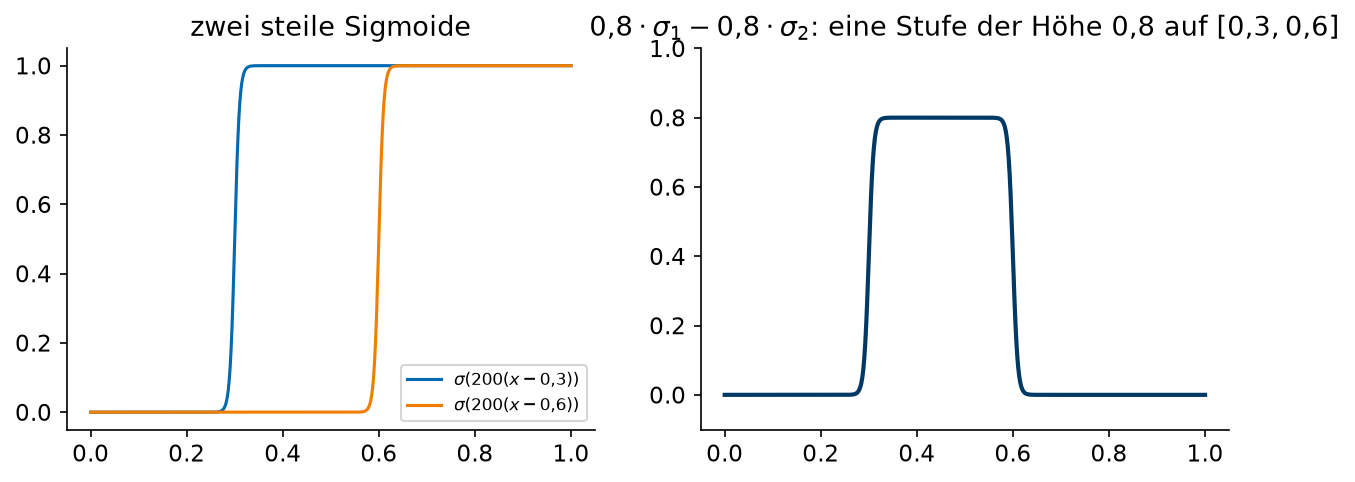
\includegraphics[width=0.62\textwidth]{vl11-step-from-sigmoids.png}
  \end{center}

  \note{Zwei steile Sigmoide, Ausgabegewichte $+h$ und $-h$: eine Stufe der Höhe $h$.
    Aus Stufen baut man Stufenfunktionen, daraus approximiert man alles Messbare.
    Konstruktion von Michael Nielsen, Kapitel 4 seines Buchs --- frei online.}
\end{frame}

\begin{frame}
  \frametitle{Präziser}

  \begin{center}
    \Large
    Pinkus / Kidger--Lyons: schmale, aber \emph{tiefe} Netze reichen\\
    {\small (Schichten der Breite $d + D + 2$)}\\[16pt]
    Yarotsky (2017): $c\log(1/\varepsilon)$ Schichten, $c\,\varepsilon^{-d/k}$ Gewichte
  \end{center}

  \note{Die Zahl der Gewichte wächst exponentiell in der Eingabedimension --- der Fluch
    der Dimensionalität. Aber: glattere Funktionen (größeres $k$) brauchen weniger, und
    die \emph{Tiefe} wächst nur logarithmisch in der Genauigkeit.
    Am Rande, wenn Zeit ist: Jedes ReLU-Netz lässt sich auch als Entscheidungsbaum
    schreiben (Aytekin 2022) --- der Baum ist allerdings exponentiell groß.}
\end{frame}

\begin{frame}
  \frametitle{Take-Home}

  \begin{center}
    \Large
    Die Gewichte \emph{existieren} --- wir haben sie hingeschrieben.\\[16pt]
    Also kann der Optimierer sie auch finden.\\[16pt]
    \normalsize Aber: Netze interpolieren gut und extrapolieren schlecht.
  \end{center}

  \note{Der letzte Satz ist die wichtigste Warnung des Kapitels: Außerhalb der Stützstellen
    wird die Approximation beliebig schlecht. So rechnet auch die GPU den Sinus --- per
    Lookup-Table mit Interpolation, und nur im vorgesehenen Bereich.}
\end{frame}

\begin{frame}
  \frametitle{Blatt 7}

  \begin{center}
    \Large Nächste Woche: Autoencoder.
  \end{center}

  \note{Blatt 7 ist die Backpropagation-Rechnung aus der letzten Woche; wer sie noch nicht
    angefangen hat, sollte das jetzt tun.
    Spielaufgabe, die bleibt: XOR im Playground mit möglichst wenigen Neuronen.}
\end{frame}

\end{document}

%%% Local Variables:
%%% mode: latex
%%% TeX-master: t
%%% End:
